\subsection{Распространение сигнала вдоль длинный линий связи. Прямая и обратные волны в линии.}

Электричекими линиями с распределенными параметрами называют такие линии, в которых для одного и того же момента времени ток и напряжение непрерывно изменяются при переходе от точки к точке, т.е. являются функциями времени и пространственной координаты.

Магнитные линии с распред. параметрами - линии, магнитный поток и магнитное напряжение вдоль которых нерперывно изменяется при переходе от одной точки линии к соседней.

Эффект непрерывного изменения тока и электрического напряжения имеет место вследствие того, что линии обладают распределенными продольными и поперечными элементами. 
\begin{center}
	\begin{figure}[h!]
		\center{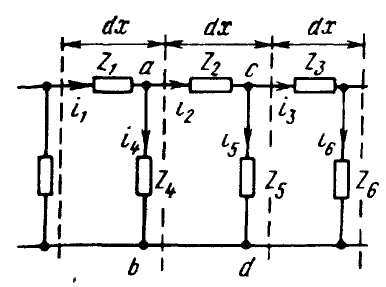
\includegraphics[scale=1.1]{l.png}}
		\caption{Изображение линии}	
		\end{figure}
\end{center}
Выше приведен участок линии с распределенными параметрами, через dx обозначен бесконечно малый элемент длины линии. 

Сопротивления $Z_{1},Z_{2},Z_{3} ...$ называют продольными, $Z_{4}, Z_{5}, Z_{6} ...$ - поперечными. 

В результате утечки тока через сопротивление $Z_4$, $i_2 != i_1$ Аналогично $U_{ab} != U_{cd}$

В электрических линиях с распределенными параметрами продольные сопротивления образованы активными сопротивлениями проводов линии и индуктивностями двух противостоящих друг другу участков линии длиной dx. Поперечные сопротивления состоят из сопротивлений утечки, появляющейся вследствие несовершенства изоляции между проводами линии и емкостей, образованных противостоящими друг другу элементами линии.

Составим дифференциальное уравнение для однородной линии с распределенными параметрами:
\begin{center}
	\begin{figure}[h!]
	\center{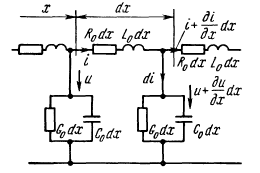
\includegraphics[scale=1]{l2.png}}
		\caption{}	
		\end{figure}
\end{center}



\begin{itemize}
\item $R_0$ - продольное активное сопротивление единицы длины линии
\item $L_0$ - индуктивность единицы длины линии
\item $C_0$ - емкость единицы длины линии
\item $G_0$ - поперечная проводимость единицы длины линии
\end{itemize}
Разобьем линию на участки dx. Если для некоторого момента $t$ ток в начале рассматриваемого участка равен $i$, то в результате утечки ток в конце участка будет равен уже $i + \frac{\partial i}{\partial x}dx$. Аналогично и для напряжения. Произведем обход по часовой стрелке для замкнутого контура, образованного участком $dx$:
$$
-u + R_0 dxi + L_0 dx\frac{\partial i}{\partial t} + u + \frac{\partial u}{\partial x} dx = 0
$$
После упрощения
$$
-\frac{\partial u}{\partial x}= L_0 \frac{\partial i}{\partial t} + R_0 i
$$
По первому закону Кирхгофа:
$$
i = di + i + \frac{\partial i}{\partial x} dx
$$
$$
di = uG_0 dx + C_0 dx\frac{\partial u}{\partial t}
$$
$$
-\frac{\partial i}{\partial x} = G_0 u + C_0 \frac{\partial u}{\partial t}
$$

Мы получили два уравнения
$$
-\frac{\partial u}{\partial x}= L_0 \frac{\partial i}{\partial t} + R_0 i
$$
$$
-\frac{\partial i}{\partial x} = G_0 u + C_0 \frac{\partial u}{\partial t}
$$
, которые являются основными дифференциальными уравнениями для линии с распределенными параметрами.

{\bfseries Решение уравнений линии.} Пусть напряжение и ток изменяются по синусоидальному закону. При использовании символического метода можно перейти от частных производных к обычным дифференциалам, т.к. Представления изображений тока и напряжения будут зависеть только от 1 параметра. Подставляя изображения в основные дифференциальные уравнения и сокращая, получаем
$$
- \frac{d\dot{U}}{dx} = Z_0 \dot{I}
$$
$$
- \frac{d\dot{I}}{dx} = Y_0 \dot{U}
$$
,где $Z_0 = R_0 + j\omega L_0 $ , $Y_0 = G_0 + j\omega C_0$ Решим эту систему относительно $\dot{U}$.
$$
-\frac{d^2 \dot{U}}{dx^2} = Z_0 \frac{d\dot{I}}{dx}
$$
Его решение 
$$
\dot{U} = \dot{A_1}e^{\gamma x} + \dot{A_2}e^{-\gamma x}
$$ Обозначим *.

Комплексное число $\gamma = \sqrt{Z_0 Y_0}$, получающееся при решении дифференциального уравнения, называют постоянной распространения.
Отношение $Z_0 /\gamma = \sqrt{Z_0 /Y_0}$, имеющее размерность сопротивления, обозначают $\rho$ и называют волновым сопротивлением.
 
{\bfseries Постоянная распространения и волновое сопротивление } 
$$
\gamma = \sqrt{(R_0 + j\omega L_0)(G_0 + j\omega C_0)}
$$
\begin{itemize}
\item Для линии постоянного тока $\omega = 0$, => $\gamma = \sqrt{R_0 G_0} $
\item Для линии синусоидального тока без потерь $R_0 = G_0 = 0$, => $\gamma = j\omega\sqrt{L_0 C_0}$
\end{itemize}
Тогда волновые сопротивления соответственно будут равны
$\rho_1 = \sqrt{R_0 / G_0} $ и $\rho_2 = \sqrt{L_0 /C_0}$
Это написано для участков линии. Для полной линии уравнения записываются аналогично. 

{\bfseries Падающие и отраженные волны}
Подставим в формулу * $A_1 e^{j\psi_0}$ вместо $A_1$ и $A_2 e^{j\psi_p}$ вместо $A_2$. Положив $\gamma = \alpha + j\beta$ и перейдя от комплексов к функциям от времени(в качестве символического изображения использовалось изображение напряжения $\dot{U} = U_m e^{j\phi_u}/\sqrt{2}$, то же, что и для решения уравнений линии), получаем
$$
u = A_1 \sqrt{2}e^{\alpha x}\sin(\omega t + \psi_0 + \beta x) + A_2\sqrt{2}e^{-\alpha x}\sin(\omega t + \psi_p - \beta x)
$$
Аналогично можно показать для тока.
$\beta$, называемый коэффициентом фазы, характеризует фазовую скорость волны $v_f = \omega/\beta$, то есть отчетливо видно, что сигнал представлен как суперпозиция набегающей и отраженной волны. $\alpha$ же называется коэффициентом затухания.
Падающей электромагнитной волной называют процесс перемещения электромагнитной волны от источника энергии к приемнику. Падающая волна несёт энергию, заключенную в ее электрическом и магнитном полях
Отражённой электромагнитной волной называют процесс перемещения электромагнитного состояния от приемника к источнику энергии.

